\section{Dataset Description}
The telemetry dataset for SmartGrid Sentinel comprises 65,983 raw observations collected across 143 unique Upazilas (spanning 15 districts) within the Sylhet and Chattogram divisions of Bangladesh. Telemetry data were sampled at 2-hour intervals across 1,000 distinct feeder channels.

Each telemetry snapshot contains 27 raw feature columns detailing datetime stamps, meteorological parameters (ambient temperature, relative humidity, rainfall, wind speed, weather condition state), and electrical grid metrics (electricity demand, renewable generation, transformer load, transformer capacity, transformer age, substation ID, feeder ID, historical outages, and industrial load ratio).

Table \ref{tab:dataset_stats} provides a comprehensive summary of the dataset attributes, spatial scope, and temporal properties.

\begin{table}[htbp]
\caption{Dataset Statistics Summary}
\centering
\resizebox{\columnwidth}{!}{%
\begin{tabular}{lc}
\toprule
\textbf{Dataset Attribute} & \textbf{Quantitative Value} \\
\midrule
Total Initial Raw Telemetry Records & 65,983 \\
Post-Target Shifting Valid Records & 64,983 \\
Geographic Scope (Upazilas) & 143 Upazilas \\
Administrative Scope (Districts) & 15 Districts \\
Substation Feeder Channels & 1,000 Feeders \\
Raw Feature Columns & 27 Features \\
Model Input Features (Engineered) & 28 Features \\
Telemetry Sampling Interval & 2 Hours \\
Historical Lookback Window ($seq\_len = 5$) & 10 Hours \\
Forecast Horizon Step & 2 Hours ($T+2\text{h}$) \\
\bottomrule
\end{tabular}%
}
\label{tab:dataset_stats}
\end{table}

The target variable, \texttt{risk\_level}, categorizes grid risk into three operational tiers: \texttt{Low} (normal operating range), \texttt{Medium} (moderate capacity stress), and \texttt{High} (severe load shedding / capacity overload risk). As illustrated in Fig. \ref{fig:class_dist}, the dataset exhibits class imbalance, with \texttt{Medium} Risk representing 75.8\% of observations ($N = 49,271$), \texttt{Low} Risk representing 13.1\% ($N = 8,502$), and \texttt{High} Risk representing 11.1\% ($N = 7,210$).

\begin{figure}[htbp]
\centering
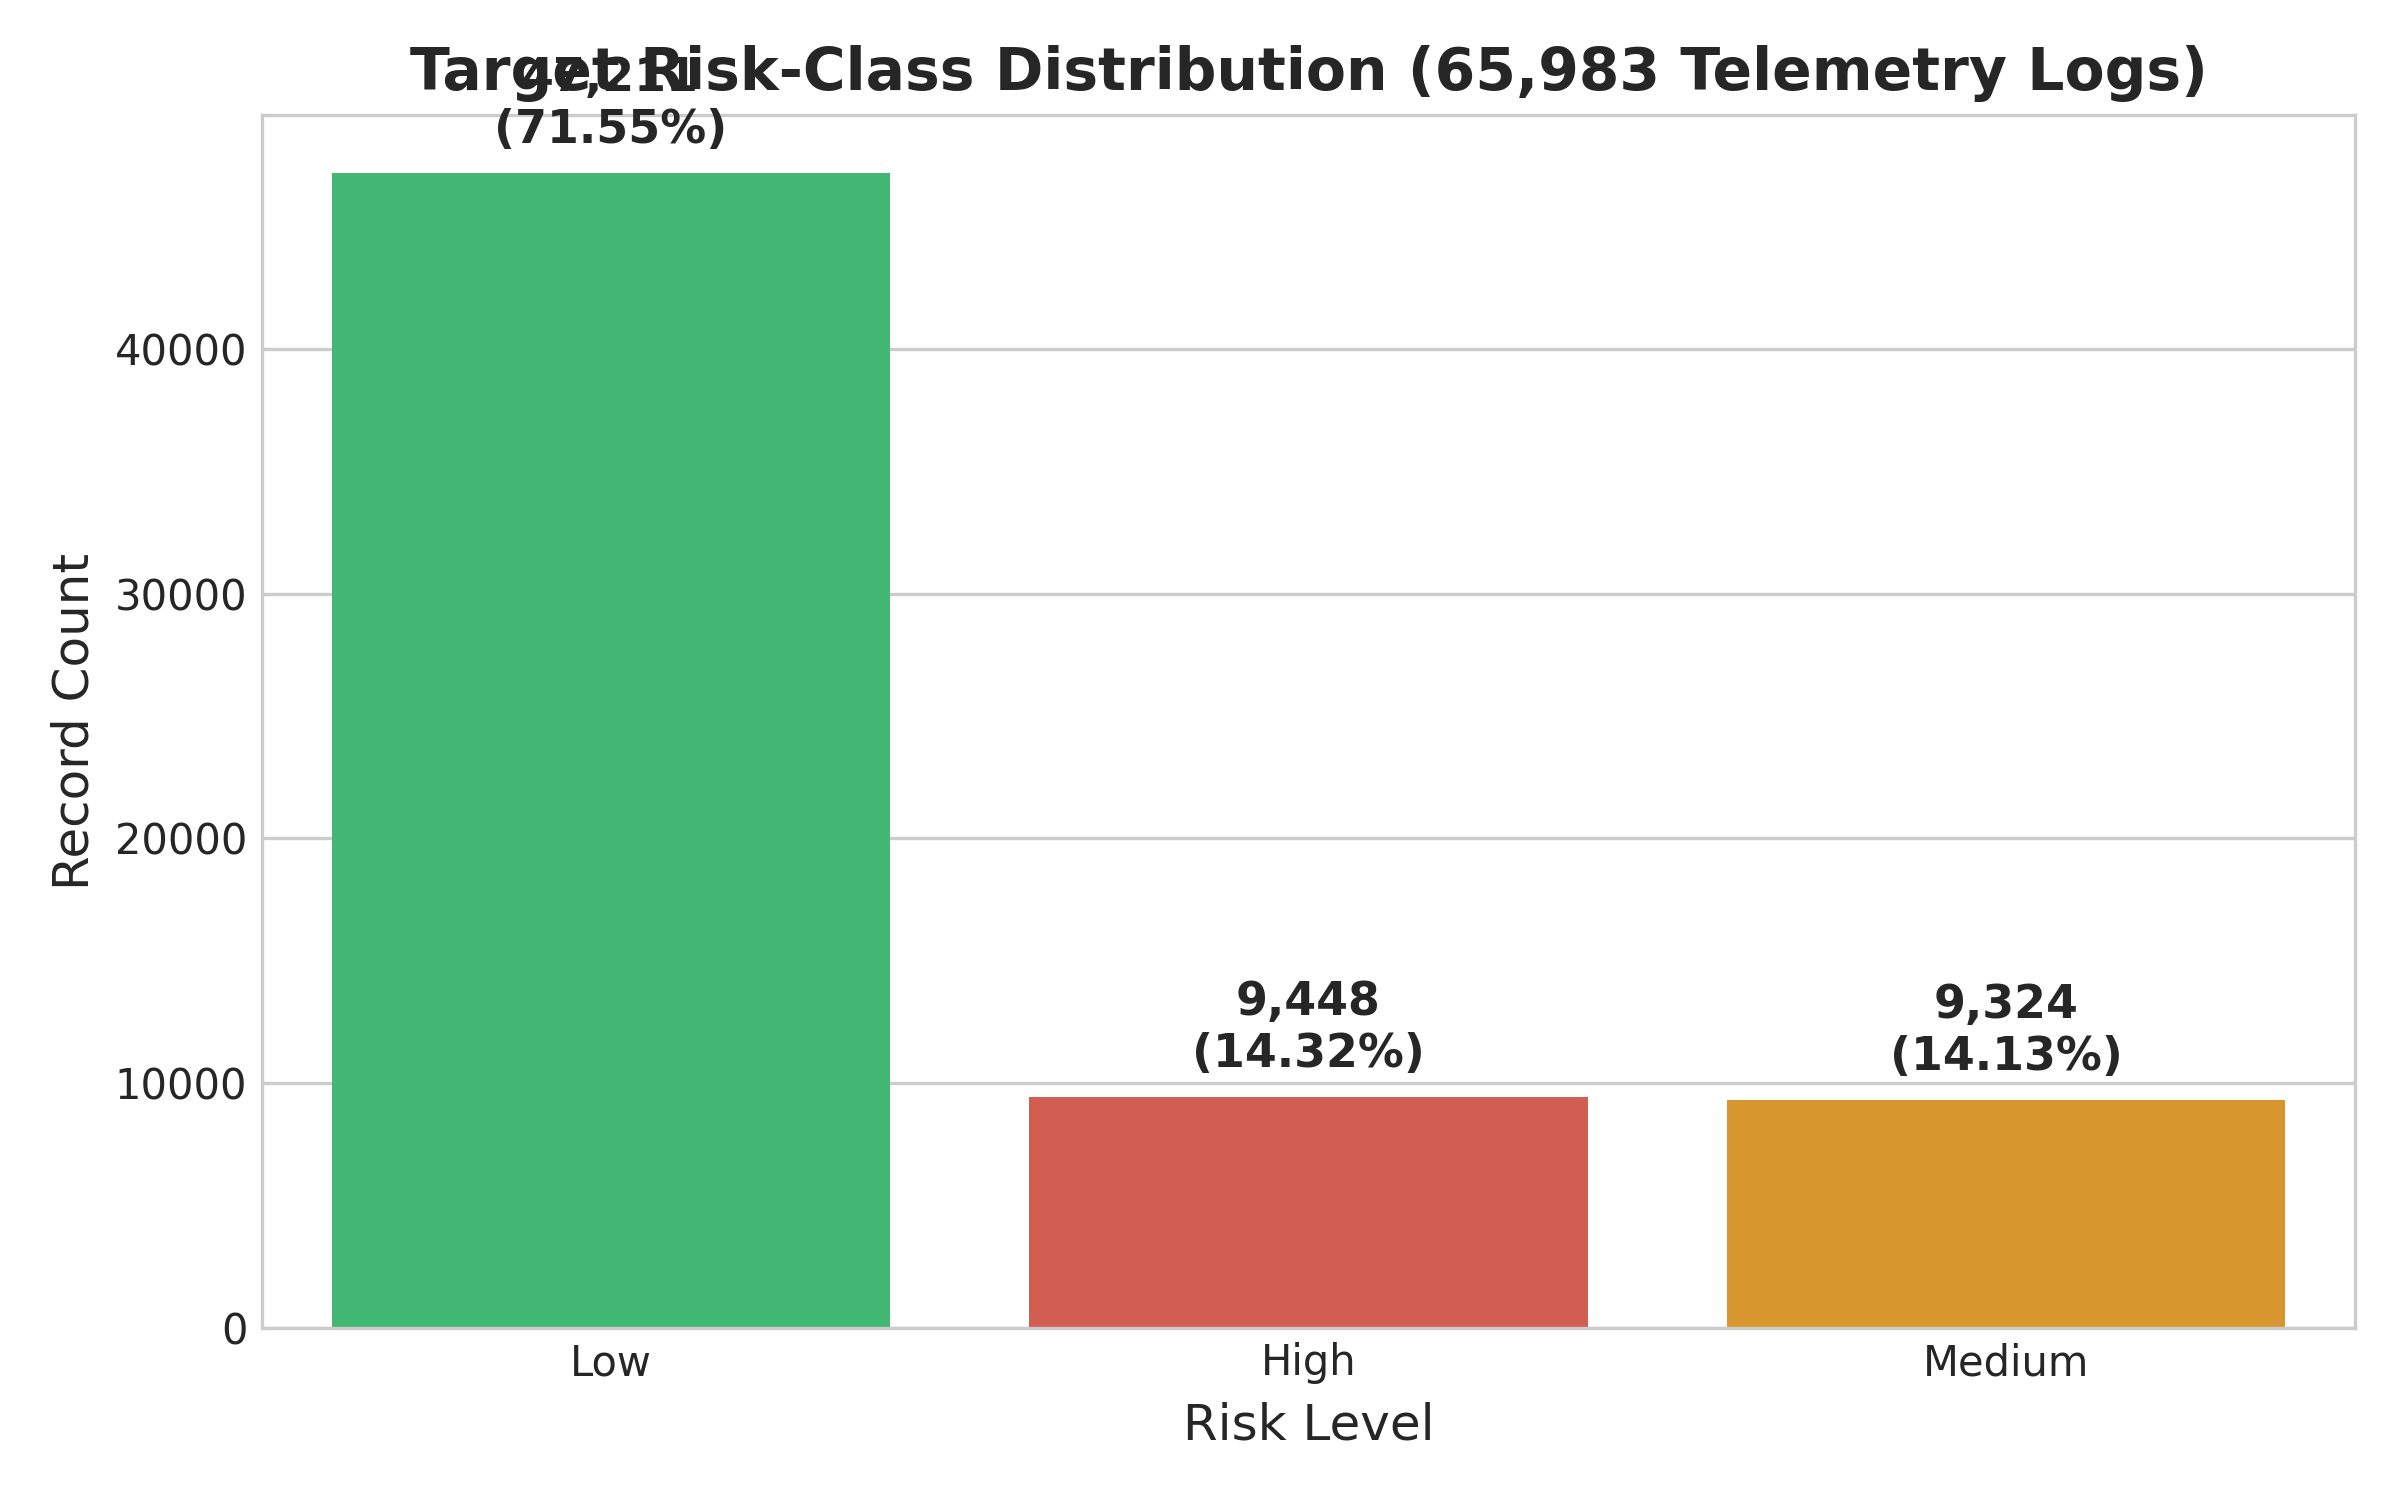
\includegraphics[width=0.85\linewidth]{figures/fig5_class_distribution.png}
\caption{Distribution of Grid Risk Classes Across Telemetry Snapshots.}
\label{fig:class_dist}
\end{figure}
